

\section{Introduction and contextualization}\label{sec:context}
This article provides context for the research conducted in Zephyr Serret Verbist's Bachelor's Thesis, undertaken at the Faculty of Informatics of Barcelona (FIB) at the Universitat Politècnica de Catalunya, under the guidance of Gabriel Valiente Feruglio. It encompasses an exploration of the research's background, the applied methodology, the rationale behind the study, and the obtained results.

\subsection{Terms and concepts used in this study}

\subsubsection{Hypergraphs}

Hypergraphs are an extension of graphs that employs hyperedges instead of edges. A hyperedge is defined by two non-empty sets of nodes: a tail set and a head set. The hyperedge models a relationship originating from all elements in its tail set to all elements in its head set, or it can be undirected.

Let us recall from~\cite{Gallo.Longo.Pallottino.Nguyen:1993} the following definition, where we impose the tail set and head set of a hyperedge to be nonempty sets of nodes.

\begin{defn}
A directed hypergraph $H=(V,E)$ consists of a set of nodes $V$ and a set of hyperedges $E=\{\ (T(e),H(e))\ \mid T(e)\ \subseteq\ V,\ H(e)\ \subseteq\ V,\ T(e)\neq\emptyset,\ H(e)\neq\emptyset\}$.
\end{defn}

\begin{figure}[H]
\centering
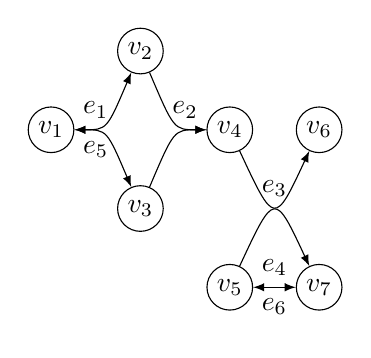
\begin{tikzpicture}[baseline,xscale=0.5675]
    \tikzstyle{every picture}=[thick]
    \tikzstyle{every node}=[inner sep=2pt,circle,draw]
    \draw (0,2) node (1) {$v_1$};
    \draw (2,3) node (2) {$v_2$};
    \draw (2,1) node (3) {$v_3$};
    \draw (4,2) node (4) {$v_4$};
    \draw (4,0) node (5) {$v_5$};
    \draw (6,2) node (6) {$v_6$};
    \draw (6,0) node (7) {$v_7$};
    \draw[latex-latex] (1) .. controls (1.25,2) .. (2);
    \draw[latex-latex] (1) .. controls (1.25,2) .. (3);
    \draw[-latex] (2) .. controls (2.75,2) .. (4);
    \draw[-latex] (3) .. controls (2.75,2) .. (4);
    \draw[-latex] (4) .. controls (5,0.78125) .. (6);
    \draw[-latex] (5) .. controls (5,1.21875) .. (7);
    \draw[latex-latex] (5) -- (7);
    \draw (1,2.25) node[draw=none] {$e_1$};
    \draw (3,2.25) node[draw=none] {$e_2$};
    \draw (5,1.25) node[draw=none] {$e_3$};
    \draw (5,0.25) node[draw=none] {$e_4$};
    \draw (1,1.75) node[draw=none] {$e_5$};
    \draw (5,-0.25) node[draw=none] {$e_6$};
\end{tikzpicture}
\caption[Example of a directed hypergraph $H=(V,E)$]
%{\tabular[t]{@{}l@{}}Example of a directed hypergraph $H=(V,E)$\\ with $V=\{v_1,v_2,v_3,v_4,v_5,v_6,v_7\}$ and $E=\{e_1,e_2,e_3,e_4,e_5,e_6\}$\\ where $e_1=(\{v_1\},\{v_2,v_3\})$, $e_2=(\{v_2,v_3\},\{v_4\})$, $e_3=(\{v_4,v_5\},\{v_6,v_7\})$,\\\hspace{24pt} $e_4=(\{v_5\},\{v_7\})$, $e_5=(\{v_2,v_3\},\{v_1\})$, $e_6=(\{v_7\},\{v_5\})$.\endtabular}
{Example of a directed hypergraph $H=(V,E)$ with $V=\{v_1,v_2,v_3,v_4,v_5,v_6,v_7\}$ and $E=\{e_1,e_2,e_3,e_4,e_5,e_6\}$, where $e_1=(\{v_1\},\{v_2,v_3\})$, $e_2=(\{v_2,v_3\},\{v_4\})$, $e_3=(\{v_4,v_5\},\{v_6,v_7\})$, $e_4=(\{v_5\},\{v_7\})$, $e_5=(\{v_2,v_3\},\{v_1\})$, $e_6=(\{v_7\},\{v_5\})$.}
\label{fig:Hypergraph-example}
\end{figure}

\subsubsection{Metabolic Pathway}
A metabolic pathway is a set of linked chemical reactions that occur in the cell.
Hypergraphs are particularly well-suited for modeling metabolic pathways because metabolic reactions often involve multiple substrates and multiple products~\cite{Pearcy.Crofts.Chuzhanova:2014}. While these reactions typically have a dominant direction, it is also possible for some reactions to proceed in the opposite direction~\cite{SORRIBAS1989239}. Figure \ref{fig:hsa00600} shows a representation of the Sphingolipid metabolic pathway map in Homo Sapiens.

\begin{figure}[H]
    \centering
    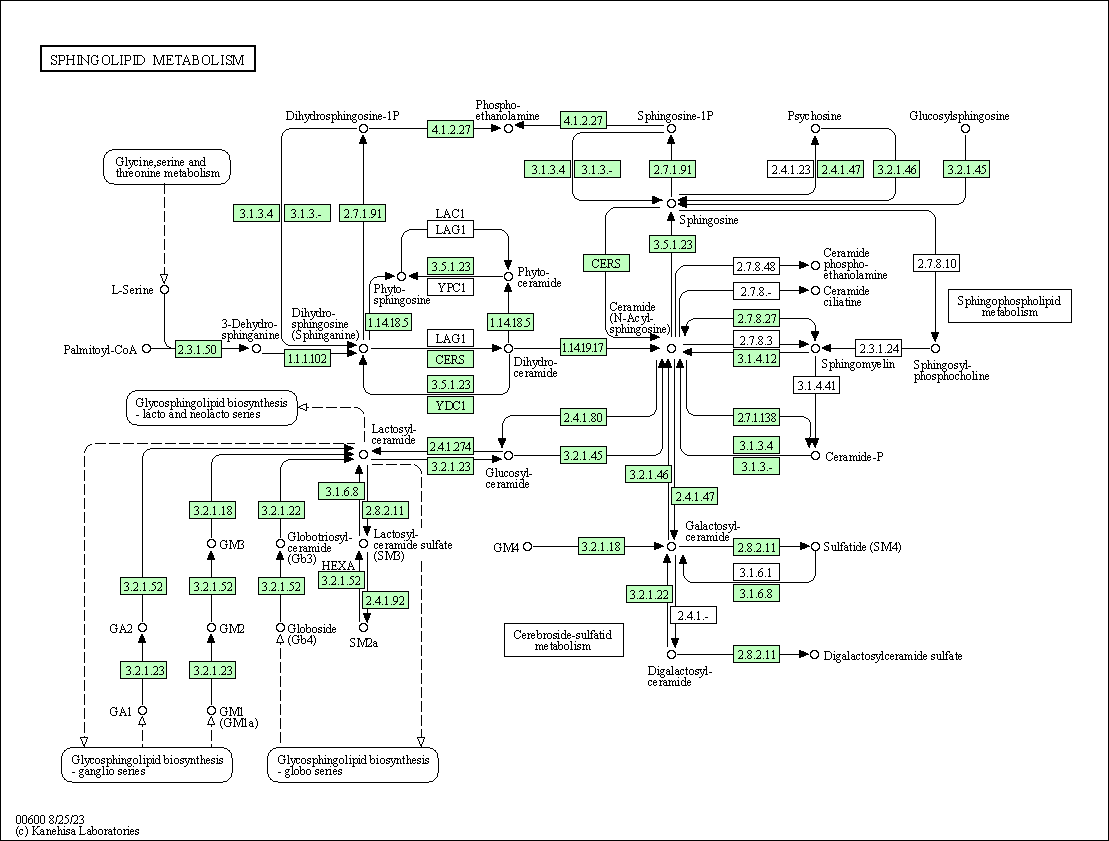
\includegraphics[width=\textwidth]{GEP1/hsa00600.png}
    \caption{Sphingolipid metabolism. Source: \href{https://www.kegg.jp/entry/map00600}{KEGG entry hsa map00600}}
    \label{fig:hsa00600}
\end{figure}

Throughout this study, we will utilize authentic metabolic pathways sourced from the Kyoto Encyclopedia of Genes and Genomes (KEGG) database. These real-world pathways will serve a dual purpose: firstly, to rigorously assess the effectiveness of our proposed solution, and secondly, to establish a robust benchmark against which future evaluations can be conducted. The determination of practical relevance and application of our results will be subject to evaluation by researchers in the field, ensuring the impartial assessment of our methodology within the context of real biological systems.

Using hypergraphs to model metabolic pathways allows us to capture the complexity and interdependencies inherent in cellular metabolism. This modeling approach provides a robust framework for studying and analyzing the intricate network of biochemical reactions that occur within cells, shedding light on the underlying processes crucial to understanding cellular function and regulation.

\subsubsection{Internal and external vertices} \label{sec:internal_external_definition}
In the context of directed graphs and hypergraphs, we introduce the concept of internal and external nodes. An internal node is defined by meeting two essential criteria: it must have an in-degree greater than zero, indicating incoming connections, and it must also have an out-degree greater than zero, signifying outgoing connections. Conversely, if a node fails to satisfy either of these criteria, it is considered external.

Applying this concept to a given metabolic pathway and its corresponding hypergraph, an internal node implies that the associated metabolite serves as both a substrate and a product within the metabolic pathway. In contrast, when a node is external, it indicates that the metabolite functions either as an input into the metabolic pathway or as a final product, thereby shedding light on the role of the metabolite in the broader context of the pathway's inputs and outputs.

\subsection{Problem definition}

In the context of undirected or partially directed hypergraphs, the objective is to determine an optimal orientation of the hyperedges that minimizes the number of external nodes. An external node is defined as a node within the hypergraph that lacks either incoming or outgoing hyperedges. To address this problem, we aim to develop an integer linear programming (ILP) model capable of finding a feasible solution within a reasonable computational timeframe.

In essence, this problem seeks to find an orientation for the hyperedges that maximizes the internal connectivity of nodes while minimizing their isolation as external nodes. The ILP model will serve as a valuable tool to achieve this goal, providing an efficient means of optimizing the orientation of hyperedges and facilitating the analysis of complex hypergraph structures.

The Figure \ref{fig:Hypergraph-orientation-example} shows two possible orientations of the hypergraph given in Figure \ref{fig:Hypergraph-example} and demonstrates the impact of the orientation on the number of external nodes.
The first orientation has 2 external nodes and the second one has 5 external nodes. The external nodes are highlighted in yellow. The first orientation is optimal in this case.

\begin{figure}[H]
    \centering
    \begin{multicols}{2}
        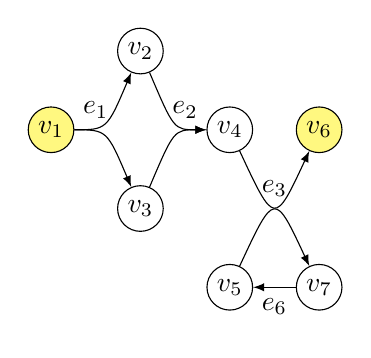
\begin{tikzpicture}[baseline,xscale=0.5675]
            \tikzstyle{every picture}=[thick]
            \tikzstyle{every node}=[inner sep=2pt,circle,draw]
            \draw (0,2) node [fill=yellow!50] (1) {$v_1$};
            \draw (2,3) node (2) {$v_2$};
            \draw (2,1) node (3) {$v_3$};
            \draw (4,2) node (4) {$v_4$};
            \draw (4,0) node (5) {$v_5$};
            \draw (6,2) node [fill=yellow!50] (6) {$v_6$};
            \draw (6,0) node (7) {$v_7$};
            \draw[-latex] (1) .. controls (1.25,2) .. (2);
            \draw[-latex] (1) .. controls (1.25,2) .. (3);
            \draw[-latex] (2) .. controls (2.75,2) .. (4);
            \draw[-latex] (3) .. controls (2.75,2) .. (4);
            \draw[-latex] (4) .. controls (5,0.78125) .. (6);
            \draw[-latex] (5) .. controls (5,1.21875) .. (7);
            \draw[latex-] (5) -- (7);
            \draw (1,2.25) node[draw=none] {$e_1$};
            \draw (3,2.25) node[draw=none] {$e_2$};
            \draw (5,1.25) node[draw=none] {$e_3$};
            \draw (5,-0.25) node[draw=none] {$e_6$};
        \end{tikzpicture}
        
        \columnbreak           
        
        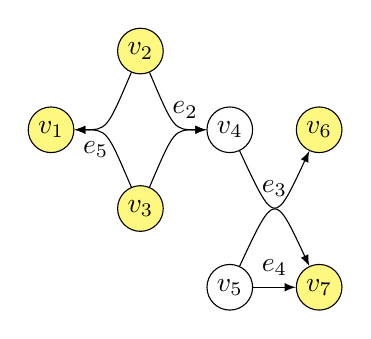
\begin{tikzpicture}[baseline,xscale=0.5675]
            \tikzstyle{every picture}=[thick]
            \tikzstyle{every node}=[inner sep=2pt,circle,draw]
            \draw (0,2) node [fill=yellow!50] (1) {$v_1$};
            \draw (2,3) node [fill=yellow!50] (2) {$v_2$};
            \draw (2,1) node [fill=yellow!50] (3) {$v_3$};
            \draw (4,2) node (4) {$v_4$};
            \draw (4,0) node (5) {$v_5$};
            \draw (6,2) node [fill=yellow!50] (6) {$v_6$};
            \draw (6,0) node [fill=yellow!50] (7) {$v_7$};
            \draw[latex-] (1) .. controls (1.25,2) .. (2);
            \draw[latex-] (1) .. controls (1.25,2) .. (3);
            \draw[-latex] (2) .. controls (2.75,2) .. (4);
            \draw[-latex] (3) .. controls (2.75,2) .. (4);
            \draw[-latex] (4) .. controls (5,0.78125) .. (6);
            \draw[-latex] (5) .. controls (5,1.21875) .. (7);
            \draw[-latex] (5) -- (7);
            \draw (3,2.25) node[draw=none] {$e_2$};
            \draw (5,1.25) node[draw=none] {$e_3$};
            \draw (5,0.25) node[draw=none] {$e_4$};
            \draw (1,1.75) node[draw=none] {$e_5$};
        \end{tikzpicture}
    \end{multicols}
    \caption{Example of the orientation of a hypergraph and its impact on its internal and external nodes.}
    \label{fig:Hypergraph-orientation-example}
\end{figure}


\subsection{Stakeholders} \label{sec:stakeholders}

In this research project, the primary stakeholders involved are as follows:
\begin{list}{}{\leftmargin=0em}
\item \textbf{Thesis Supervisor and Team}: The thesis supervisor and their team play a pivotal role as stakeholders in this endeavor, and they are poised to benefit significantly from the study's success. Their guidance, mentorship, and valuable insights contribute significantly to the project's progress. Moreover, their team, concurrently tackling a similar problem, presents opportunities for collaboration and knowledge sharing that enrich our collective efforts. The success of this research not only advances our academic pursuits but also enhances the knowledge and expertise of our thesis supervisor and their team, positioning them at the forefront of cutting-edge research in this field.
\item \textbf{Biologists and Researchers in Life Sciences:} While the biological relevance of the project's results is still under evaluation, biologists and researchers in the field of life sciences stand to benefit from the outcomes of this research. The potential implications of the project's findings for understanding and modeling complex biological systems, particularly in the context of metabolic pathways, hold promise for these stakeholders. The insights generated by the hypergraph orientation techniques developed in this project may open new avenues for their own research and analysis, ultimately benefiting the broader scientific community.
\end{list}

\section{Justification}
In the realm of network science and analysis, the topological characterization of complex networks has been a focal point of research and investigation over the past decade. However, the analogous theory for complex hyper-networks has not seen the same level of development and attention~\cite{Pearcy.Crofts.Chuzhanova:2014}. Notably, there exists a critical gap in the field: the lack of a known polynomial-time algorithm for the optimal hypergraph orientation problem, and the computational complexity of this problem remains an open question.

To address this challenge, we have made the deliberate choice to employ Integer Linear Programming (ILP) as our optimization technique. ILP offers a powerful and versatile framework for tackling complex combinatorial problems. Given the uncharted terrain surrounding hypergraph orientation, the adaptability and precision of ILP provides a promising avenue for addressing this computational challenge and advancing our understanding of complex hyper-networks. Through ILP, we aim to explore and optimize hypergraph orientations, thereby contributing to the development of solutions in this less-explored but highly significant area of network theory.

\section{Scope}

\subsection{Objective}

The overarching objective of this research project is to develop an Integer Linear Programming (ILP) model for optimizing the orientation of hyperedges within undirected or partially directed hypergraphs. Additionally, we aim to create a user-friendly software application that seamlessly connects to the Kyoto Encyclopedia of Genes and Genomes (KEGG) database. This application will retrieve metabolic pathway entries from KEGG and interface with the ILP model to assess its efficacy in minimizing external nodes. The combined goal is to provide a powerful and practical tool for researchers to analyze and optimize hypergraph orientations within the context of real-world biological pathways.

\subsection{Sub-objectives}

\begin{enumerate}
    \item \textbf{Mathematical Model Formulation:} Define and refine the ILP model, taking into account hypergraph structures and orientation optimization criteria. This includes specifying decision variables, constraints, and the objective function.
    \item \textbf{Algorithm Development:} Implement the ILP model as a computational algorithm capable of optimizing hypergraph orientations efficiently and accurately.
    \item \textbf{Database Integration:} Create a module within the software application to connect to the KEGG database, retrieve metabolic pathway data, and format it for use in the ILP model.
    \item \textbf{User Interface Design:} Develop an intuitive and user-friendly interface for the application, enabling researchers to interact with the ILP model and KEGG database seamlessly.
    \item \textbf{Application Development:} Build the software application, integrating the ILP algorithm, database connectivity, and user interface components into a cohesive tool.
    \item \textbf{Testing and Validation:} Rigorously test the ILP model and the application using synthetic and real-world hypergraphs and metabolic pathway data from KEGG. Validate results against ground truth data where available.
    \item \textbf{Performance Optimization:} Optimize the ILP model and application for computational efficiency and scalability, ensuring it can handle large-scale hypergraphs and databases. This includes benchmarking multiple ILP models and solvers to identify the best configuration in terms of speed and accuracy.
    \item \textbf{Documentation and User Guides:} Prepare comprehensive documentation and user guides for the application, making it accessible to a wide range of researchers and practitioners.
    \item \textbf{Deployment and Accessibility:} Make the software application accessible to the research community through appropriate channels, ensuring it is readily available for use.
\end{enumerate}

\subsection{Identification of Functional and Non-Functional Requirements:}

In addition to the primary objectives and subtasks, it is imperative to identify both functional and non-functional requirements to guide the development and evaluation of the ILP model and application:

\subsubsection{Functional requirements}

\begin{enumerate}
    \item \textbf{Data Retrieval:} The application must seamlessly retrieve metabolic pathway data from the KEGG database, allowing users to specify search criteria and obtain relevant results.
    \item \textbf{Hypergraph Orientation:} The ILP model should accurately optimize hypergraph orientation, minimizing the number of external nodes while preserving the integrity of the data.
    \item \textbf{User Interface:**} The user interface should provide an intuitive and interactive platform for users to input hypergraphs, set parameters, and visualize results.
    \item \textbf{Performance:} The application should execute efficiently, providing timely results for both small and large-scale hypergraphs. It should also handle multiple ILP models and solvers for benchmarking.
    \item \textbf{Result Presentation:} The application should present orientation results in a clear and interpretable manner, enabling users to understand the impact of the orientation on the hypergraph.
\end{enumerate}

\subsubsection{Non-Functional Requirements:}
\begin{enumerate}
    \item \textbf{Usability:} The user interface should be user-friendly, with clear instructions and an intuitive design to accommodate users with varying levels of expertise.
    \item \textbf{Maintainability:} Develop the application and ILP model using good programming practices, allowing for updates, bug fixes, and future enhancements.
    \item \textbf{Scalability:} Ensure that the ILP model and application can scale to accommodate the growing volume and complexity of hypergraphs and databases.
    \item \textbf{Documentation:} Provide comprehensive documentation, including user guides, technical manuals, and developer resources to support users and maintainers.
\end{enumerate}

\subsection{Risk assessment}
In the pursuit of this research project, several significant risks have been identified, each with the potential to impact the successful completion of the objectives. Mitigating these risks is essential to maintain the project's timeline and ensure the achievement of its goals. The following risks have been identified as particularly relevant:
\begin{enumerate}
    \item \textbf{Project Timeline:} Unforeseen issues, delays in data acquisition, or unexpected complexities may pose a risk to the project's timeline and the timely achievement of milestones.\\
        \textit{Mitigation:} Develop a realistic project timeline, monitor progress regularly, and have contingency plans in place to address any delays or setbacks that may arise.
    
    \item \textbf{Computational Power:} The computational demands of solving complex ILP models, especially for large hypergraphs, may exceed available computational resources, potentially affecting the project's efficiency.\\
        \textit{Mitigation:} Get access to the computing cluster of the Department of Computer Science.
    
    \item \textbf{Integration Challenges:} Developing an application that seamlessly interfaces with the KEGG database may encounter challenges related to database structure changes, API updates, or connectivity issues.\\
        \textit{Mitigation:} Stay informed about KEGG updates, establish communication channels with the KEGG team if possible, and have a plan in place to adapt the application to accommodate changes as they occur.
    
    \item \textbf{Inexperience with ILP:} Limited prior experience or familiarity with Integer Linear Programming (ILP) modeling may present a challenge in developing and implementing effective ILP models for hypergraph orientation.
\end{enumerate}

\section{Methodology: Kanban for Solo Development} \label{sec:Methodology}

For this research project, the Kanban methodology has been selected as the ideal approach to guide the development process. 

\subsection{Adapting Kanban for Solo Development:}

In the absence of changing client priorities, Kanban will be customized to align with the solo development setting:

\smallsmalltitle{Visual Task Management:}

For efficient task management and to implement the Kanban methodology, we will leverage the Trello platform as my primary tool. Trello's user-friendly interface and visual board system make it well-suited for organizing and tracking the progress of research tasks. Within Trello, We will create dedicated boards that represent various project stages, such as ``To-Do", ``In Progress", and ``Completed". Each task or research activity will be represented as a card within the corresponding board column. This approach will provide a clear, real-time visualization of the project's workflow and enable me to maintain a structured and organized development process throughout the project's lifecycle.

\smallsmalltitle{Work in Progress (WIP) Limits:} 

Kanban's WIP limits will be employed to control the number of concurrent tasks in progress. By setting limits on work items, the development process is streamlined, preventing overloading and maintaining a manageable pace of work.

\smallsmalltitle{Continuous Monitoring:} 

Scheduled bi-weekly meetings with the thesis supervisor will serve as checkpoints for evaluating progress and addressing challenges. In addition, we will maintain consistent email communication with the supervisor. To enhance transparency and provide real-time access to project progress, all code will be hosted on a public Git repository. This repository offers version control, data backup in case of hardware failure, and potential future collaboration. It will feature a single main branch for streamlined development and marked releases to signify project milestones.

\smallsmalltitle{Feedback and Iteration:} A fundamental principle of Kanban is continuous improvement. Feedback obtained from supervisor meetings and self-assessment will guide adjustments to the project plan. This iterative approach allows for refinements in task prioritization and resource allocation as the project evolves.

\subsection{Benefits of Kanban for Solo Development:}

\begin{list}{}{\leftmargin=0em}
    \item \textbf{Efficiency:} Kanban promotes efficient task management, ensuring that effort is directed toward high-priority items.
    \item \textbf{Visibility:} The visual nature of Kanban provides a clear overview of project progress and pending tasks.
    \item \textbf{Adaptability:} Kanban's flexibility allows for seamless adjustments to the project plan based on evolving needs or new insights.
    \item \textbf{Reduced Overhead:} As a solo developer, Kanban minimizes the overhead associated with more complex project management methodologies.
\end{list}

